\documentclass[11pt,letterpaper]{article}
\PassOptionsToPackage{hyphens}{url}
\usepackage[margin=.83in,top=.8in,bottom=.8in,headheight=15pt]{geometry}
\usepackage[T1]{fontenc}
\usepackage{lmodern,amsmath,amssymb,mathtools,bm,booktabs,array,graphicx,tikz}
\usetikzlibrary{arrows.meta,positioning,calc,decorations.pathreplacing,patterns}
\definecolor{ink}{HTML}{17344D}\definecolor{accent}{HTML}{087E8B}\definecolor{pale}{HTML}{EDF5F5}\definecolor{gold}{HTML}{AD6B19}
\providecommand{\dd}{\,\mathrm{d}}\providecommand{\R}{\mathbb{R}}
\providecommand{\E}{\mathbb{E}}\providecommand{\Var}{\operatorname{Var}}
\providecommand{\Cov}{\operatorname{Cov}}\providecommand{\diag}{\operatorname{diag}}
\providecommand{\norm}[1]{\left\lVert#1\right\rVert}
\providecommand{\abs}[1]{\left|#1\right|}
\usepackage{microtype,hyperref,fancyhdr,enumitem,amsthm,sectsty,needspace}
\allsectionsfont{\raggedright}
\hypersetup{colorlinks=true,linkcolor=ink,urlcolor=accent,pdfauthor={Zan Ahmad},pdftitle={Implicit pressure equations and ideal-valve complementarity / Lecture notes}}
\setlength{\parindent}{0pt}\setlength{\parskip}{6pt}\linespread{1.07}
\setlist{itemsep=3pt,topsep=4pt,leftmargin=*}
\emergencystretch=2em\clubpenalty=10000\widowpenalty=10000
\pagestyle{fancy}\fancyhf{}\fancyhead[L]{\small Computational Cardiology}\fancyhead[R]{\small Lecture 3}
\fancyfoot[L]{\footnotesize Zan Ahmad}\fancyfoot[R]{\footnotesize\thepage}\renewcommand{\headrulewidth}{.3pt}
\newtheorem{proposition}{Proposition}\newtheorem{theorem}{Theorem}\newtheorem{lemma}{Lemma}
\theoremstyle{definition}\newtheorem{definition}{Definition}\newtheorem{example}{Example}
\numberwithin{equation}{section}
\begin{document}
{\small\scshape Computational Cardiology\hfill Lecture 3}\par\medskip
{\raggedright\hyphenpenalty=10000\exhyphenpenalty=10000\LARGE\bfseries\color{ink} Implicit pressure equations and ideal-valve complementarity\par}\medskip
{\small Lecture notes}\par\bigskip
A time-varying compliance changes pressure even when no blood enters a compartment. Discretizing stored volume directly preserves this effect and produces a coupled pressure system. Ideal valves then impose inequalities on that system; conservation alone does not determine the admissible valve state.

\section{Differentiating the constitutive storage law}
\hypertarget{note-differentiating-the-constitutive-storage-law}{}\label{note:differentiating-the-constitutive-storage-law}
{\small \href{slides.html\#frame=the-stored-quantity\&step=1}{Slides for this section}}\par
The baseline showed that matched compliance and pressure reconstruct a conserved total. We now derive the update that makes that account possible. For one compartment, $V=V_d+CP$ with constant unstressed volume Vd. Inflow minus outflow changes V. If compliance varies with cardiac phase, the continuous derivative is C times the pressure derivative plus pressure times the compliance derivative. Keeping only C times the pressure derivative would treat the moving pressure-volume relation as if it were fixed.

A simple isolation experiment reveals the missing term. Close every connection to a compartment so its volume cannot change. If its compliance halves while Vd is fixed, its pressure must double to preserve CP. An equation that sets the pressure derivative to zero because net flow is zero gives the wrong result. This observation motivates discretizing the stored quantity CP directly. It also distinguishes an active compliance change from blood entering the region.

In the six-region circulation, only ventricular compliances vary; the vascular compliances remain fixed. The phase and compliance at the next time are prescribed before the hydraulic solve. For fixed-rate pacing the phase is known directly from elapsed time. A later feedback calculation modifies how that phase is advanced, but the hydraulic balance still needs the old and new compliances rather than a substitute constant value.

\[
\dot V_i=C_i\dot P_i+\dot C_iP_i=Q_{{\rm in},i}-Q_{{\rm out},i}
\]
Vd is constant; both terms on the left have L/min.

\[
C_i^{n+1}P_i^{n+1}-C_i^nP_i^n=h\,(Q_{{\rm in},i}^{n+1}-Q_{{\rm out},i}^{n+1})
\]
Backward Euler evaluates the hydraulic flows at the new pressures; h is in minutes.

For an isolated compartment, $CP$ is constant and therefore
\[
 \frac{\dot P}{P}=-\frac{\dot C}{C},\qquad
 P^{n+1}=\frac{C^n}{C^{n+1}}P^n.
\]
The finite-step relation is exact for this isolated storage constraint, regardless of how rapidly the prescribed compliance changes.
\section{The conductance Laplacian and pressure matrix}
\hypertarget{note-the-conductance-laplacian-and-pressure-matrix}{}\label{note:the-conductance-laplacian-and-pressure-matrix}
{\small \href{slides.html\#frame=discretize-stressed-volume\&step=1}{Slides for this section}}\par
An open resistor from i to j carries the pressure difference divided by its resistance. With conductance g=1/R, the contribution to i's net outflow is g(Pi\ensuremath{-}Pj). Its contribution to j is the negative of that amount. After multiplying by h and moving new-pressure flow terms to the left, an active connection adds hg to the two diagonal entries and \ensuremath{-}hg to the two off-diagonal entries. Each term has compliance units L/mmHg, matching the diagonal storage coefficient.

The old right-hand side is old compliance times old pressure, with units liters. The new diagonal storage uses new compliance. For a given valve-state guess, each open valve contributes its conductance and each closed valve contributes zero. Vascular resistance beds remain active open resistors. Their signed flows are not clipped. The resulting simultaneous equations determine the new pressures together; the process is not a sequence of independent explicit pressure updates.

Using an incidence matrix makes the shared structure visible. Give each link a column with \ensuremath{-}1 at its source and +1 at its receiver. With diagonal active conductances G, the conductance Laplacian is B G B\ensuremath{^{\mathsf T}}. The pressure matrix is diagonal new compliance plus h times that Laplacian. Positive compliances make the storage contribution strictly positive, and nonnegative conductances add a nonnegative quadratic form. This explains why a fixed-state system has a well-posed linear solve under the stated assumptions. A matrix solve still does not establish that the guessed valves were physically consistent.

\[
[\operatorname{diag}(C^{n+1})+h B G B^{\mathsf T}]P^{n+1}=\operatorname{diag}(C^n)P^n
\]
B has \ensuremath{-}1 at each link source and +1 at its receiver; G contains current active conductances.

For any nonzero vector $z$,
\[
 z^{\mathsf T}(D_C+hBGB^{\mathsf T})z
   =\sum_iC_i z_i^2+h\sum_e g_e(z_{\rm head(e)}-z_{\rm tail(e)})^2>0.
\]
Thus the fixed-state matrix is symmetric positive definite when $C_i>0$, $h\ge0$ and active conductances are nonnegative. The pressure solution is unique for each valve configuration; the remaining problem is to select a configuration consistent with that solution.
\section{Ideal valves as a complementarity condition}
\hypertarget{note-ideal-valves-as-a-complementarity-condition}{}\label{note:ideal-valves-as-a-complementarity-condition}
{\small \href{slides.html\#frame=the-ideal-valve-law\&step=1}{Slides for this section}}\par
An ideal forward valve has flow max(Pup\ensuremath{-}Pdown,0)/R. If a valve is guessed open, the solved forward pressure difference must be nonnegative. If it is guessed closed, that difference must be nonpositive. At equality the physical flow is zero and either discrete label can represent the same state. The decisive test is the solved pressure difference, not the pressure difference before the time step.

The algorithm is therefore a coupled logic-and-pressure calculation. Choose an initial valve guess, assemble and solve the linear system, calculate new pressure differences, update any inconsistent valve states and solve again. Accept only a state that satisfies both the compartment balances and all ideal-valve conditions. In the six-compartment teaching implementation there are four valves, hence only sixteen possible configurations. The bounded iteration can check unvisited configurations if necessary and raises an error if no consistent step is obtained.

It is tempting to solve once, clip any negative reported valve flow, and continue. That changes the flow without recomputing the pressure balance that generated it. The accepted pressures may then disagree with the displayed flows. Instead, treat a changed valve state as a changed matrix and solve again. Similarly, changing resistance requires recomputing the conductance used in both the solve and the reported flow. Cached values from an earlier parameter setting can make two outputs describe different models.

\[
Q_{\rm valve}=\max(P_{\rm up}-P_{\rm down},0)/R
\]
Open: pressure difference \ensuremath{\ge}0; closed: pressure difference \ensuremath{\le}0; equality gives zero flow.

With $d=P_{\rm up}-P_{\rm down}$, the positive-part rule is equivalent to
\[
 q\ge0,\qquad Rq-d\ge0,\qquad q(Rq-d)=0.
\]
If $q>0$, the last equation forces $Rq=d$. If $q=0$, the second inequality requires $d\le0$. At $d=0$ the open and closed labels represent the same zero flow. This is a complementarity relation, rather than an independently prescribed switching schedule.
\section{A two-compartment active-set calculation}
\hypertarget{note-a-two-compartment-active-set-calculation}{}\label{note:a-two-compartment-active-set-calculation}
{\small \href{slides.html\#frame=a-rejected-closed-candidate-panel-1\&step=1}{Slides for this section}}\par
The worked reduction has two closed storage regions connected only by one forward valve. Unstressed volumes are set to zero for transparent arithmetic. Old pressures are 12 and 4 mmHg; old compliances are 0.02 and 0.03 L/mmHg. Thus old stressed volumes are 0.24 and 0.12 L. During one prescribed compliance step they change to 0.01 and 0.04 L/mmHg. Use h=0.02 min and valve resistance 2 mmHg min/L.

Begin with a closed-valve guess. No transfer occurs, so each old stressed volume is divided by its new compliance: the candidate pressures are 24 and 3 mmHg. Their sum of stored volumes is still 0.36 L. However, the forward pressure difference is 21 mmHg, which is inconsistent with a closed ideal valve. Conservation has passed while the valve rule has failed. This is the lesson's central counterexample.

For the open guess, $h/R=0.01$ L/mmHg. The two balance equations are
\[\begin{aligned}.02P_1-.01P_2&=.24,\\-.01P_1+.05P_2&=.12.\end{aligned}\] Solving gives P1=44/3 and P2=16/3 mmHg. The forward difference is 28/3 mmHg, so flow is 14/3 L/min. The transfer is hQ=7/75 L, approximately 0.093333 L. New volumes are 11/75 and 16/75 L; they total 0.36 L and their changes equal the same internal transfer with opposite signs. The open state is consistent and can be accepted.

The plotted trace shows old state, rejected closed candidate and accepted open candidate. Both candidate volume columns have the same total, which makes the insufficiency of conservation visible. The reduction demonstrates the algebra used inside the larger circulation, but its closed boundary is distinct from the public feedback paper's two storage compartments and external reservoirs. Similar compartment counts do not establish model identity.

The accepted open-state matrix is
\[
 \begin{pmatrix}.02&-.01\\-.01&.05\end{pmatrix}
 \begin{pmatrix}P_1\\P_2\end{pmatrix}
 =\begin{pmatrix}.24\\.12\end{pmatrix}.
\]
Its solution $(44/3,16/3)$ has $d=28/3>0$ and $q=d/2=14/3$. The pressure solve, storage change and valve rule therefore describe the same transfer.

\paragraph{Calculation.} Starting from the given old state and changing compliances, test the closed guess and revise it.

Old stressed volumes: 0.02\ensuremath{\times}12=0.24 L and 0.03\ensuremath{\times}4=0.12 L.

Closed guess: P=(24,3) mmHg; forward difference 21 mmHg makes it inconsistent.

Open matrix is [[0.02,\ensuremath{-}0.01],[\ensuremath{-}0.01,0.05]] L/mmHg, with right-hand side (0.24,0.12) L.

Accepted P=(44/3,16/3) mmHg; Q=14/3 L/min; transferred volume=7/75 L.

New volumes 11/75 and 16/75 L sum to 0.36 L, and both compartment residuals vanish to rounding.

Accept the open solve only after both balance and valve checks pass.
\begin{center}\begin{minipage}{.98\linewidth}\centering
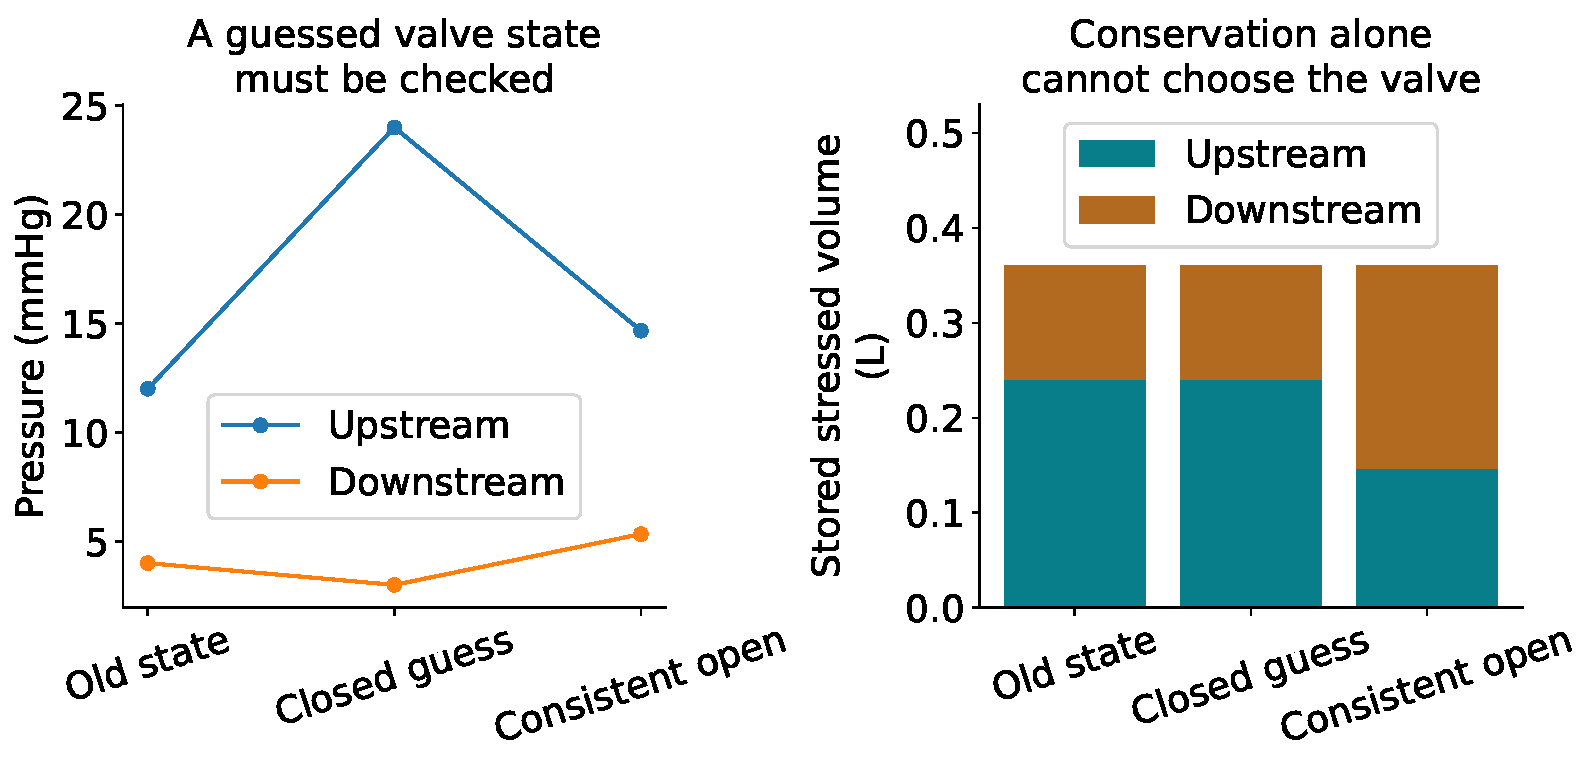
\includegraphics[width=.96\linewidth,height=.57\textheight,keepaspectratio]{valve-trace.pdf}\par\smallskip
{\small Closed two-storage worked reduction with changing compliances. The rejected closed guess and accepted open solve both conserve 0.36 L; only the latter obeys the ideal-valve pressure condition.}
\end{minipage}\end{center}
\section{Exact relaxation and backward-Euler error}
\hypertarget{note-exact-relaxation-and-backward-euler-error}{}\label{note:exact-relaxation-and-backward-euler-error}
{\small \href{slides.html\#frame=constant-compliance-relaxation\&step=1}{Slides for this section}}\par
Conservation and valve consistency do not make backward Euler exact. To isolate its time error, hold both compliances constant and start with upstream pressure above downstream pressure, so the valve stays open during relaxation. Let $d=P_1-P_2$. The first balance gives $\mathrm dP_1/\mathrm dt$=$-d/(RC_1)$, and the second gives $\mathrm dP_2/\mathrm dt$=$d/(RC_2)$. Subtracting yields an exponential decay for d with rate $(1/C_1+1/C_2)/R$. The conserved stressed volume sets the common limiting pressure.

The companion uses $C_1=0.01$, $C_2=0.04$ L/mmHg, R=2 mmHg min/L and initial pressures 20 and 5 mmHg. The conserved stressed volume is 0.4 L and the limiting pressure is 8 mmHg. The decay rate is 62.5 per minute. The upstream exact solution is $8+12e^{-62.5t}$. Compare backward-Euler runs at the same final physical time, 0.08 min, using steps 0.02, 0.01 and 0.005 min. In the author run the upstream endpoint errors decrease from about 0.387 to 0.166 to 0.074 mmHg.

These controlled cases test the implementation against a separately derived solution. They do not establish the same convergence behavior across every switching event in a six-compartment feedback model. The exact curve belongs to constant compliance and an open valve; applying it across prescribed compliance changes would compare different problems. Keep model assumptions fixed while changing only numerical resolution.

\[
\dot d=-\lambda d,\qquad \lambda=(1/C_1+1/C_2)/R
\]
This reference requires constant compliances and an open valve.

\[
d^{n+1}=d^n/(1+h\lambda)
\]
The multiplier lies between zero and one for $h>0$ and $\lambda>0$, but differs from $e^{-h\lambda}$.

For fixed compliances and an open connection, the common limiting pressure is
\[
 P_\infty=\frac{C_1P_1(0)+C_2P_2(0)}{C_1+C_2}.
\]
Backward Euler gives $d_{n+1}=d_n/(1+h\lambda)$, whereas the exact factor is $e^{-h\lambda}$. Their logarithms differ by $\tfrac12(h\lambda)^2+O(h^3)$ per step. Over a fixed interval, accumulation produces first-order global error in this smooth relaxation problem.
\begin{center}\begin{minipage}{.98\linewidth}\centering
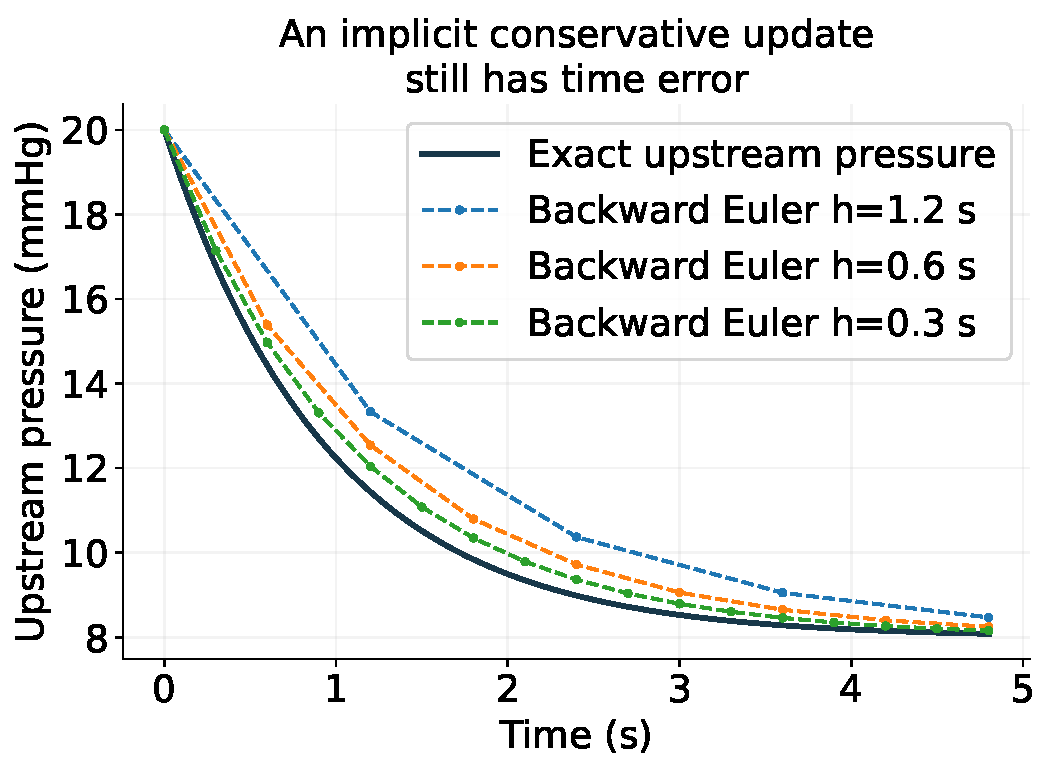
\includegraphics[width=.96\linewidth,height=.57\textheight,keepaspectratio]{implicit-refinement.pdf}\par\smallskip
{\small Constant-compliance open-valve relaxation. Backward-Euler trajectories approach an independently derived exponential solution as the step decreases.}
\end{minipage}\end{center}
\section{Extension to the six-compartment circuit}
\hypertarget{note-extension-to-the-six-compartment-circuit}{}\label{note:extension-to-the-six-compartment-circuit}
{\small \href{slides.html\#frame=conservation-and-admissibility\&step=1}{Slides for this section}}\par
The full circuit repeats the same storage and link assembly for six pressure unknowns. The four valve labels create the state-consistency problem; two tissue beds stay active. Summing all six accepted balance rows cancels the active conductance terms and preserves the initialized total. The pressure solve and the valve check should therefore be exposed as separate diagnostics even though they belong to one accepted time step.

Carry three questions into the feedback lesson: does the clock supply consistent new compliances to both ventricles, does the current resistance enter both solving and reporting, and do hydraulic balance and valve conditions pass after every step? The controller and pressure filter add their own update equations. They do not turn this hydraulic solver into explicit Euler, nor can they repair a pressure step accepted with inconsistent valves.

For four valves, exhaustive enumeration contains only $2^4=16$ configurations. Each candidate requires a positive-definite linear solve followed by four sign tests. A faster active-set iteration can reuse the preceding configuration, but it must still reject any candidate that fails the new-pressure inequalities. Summing accepted balances preserves total volume because the active conductance Laplacian always has zero row sums.
\bigskip
\section*{Exercises}
\par\noindent\begin{minipage}{\linewidth}
\subsection*{A3-1. An isolated pumping compartment}
A sealed region has Vd=\allowbreak{}0.03 L, initial C=\allowbreak{}0.02 L/mmHg and initial P=\allowbreak{}8 mmHg. C changes to 0.008 L/mmHg with no flow.

\textbf{a} Find total volume and the final pressure required by conservation.

\end{minipage}\par\medskip
\textbf{b} What error results if pressure is incorrectly held at 8 mmHg?

\textbf{c} Identify the missing continuous-balance term.

\par\noindent\begin{minipage}{\linewidth}
\subsection*{A3-2. A new valve trace}
Two closed regions have constant compliances C1=\allowbreak{}C2=\allowbreak{}0.02 L/mmHg, initial P=\allowbreak{}(18,6) mmHg, R=\allowbreak{}1 mmHg min/L, h=\allowbreak{}0.01 min and zero unstressed volumes.

\textbf{a} Test a closed initial guess.

\end{minipage}\par\medskip
\textbf{b} Assemble and solve the open system.

\textbf{c} Calculate flow and check both volumes and the total.

\par\noindent\begin{minipage}{\linewidth}
\subsection*{A3-3. Check a proposed update beyond its total}
Use the data in A3-2. A proposed code uses old flow (18-6)/1=\allowbreak{}12 L/min for the transfer, obtaining new pressures (12,12) mmHg.

\textbf{a} Does the proposed update conserve total volume?

\end{minipage}\par\medskip
\textbf{b} Does it solve the stated backward-Euler system?

\textbf{c} How should the result be described or repaired?

\par\noindent\begin{minipage}{\linewidth}
\subsection*{A3-4. A reference with explicit assumptions}
Two constant compliances are C1=\allowbreak{}C2=\allowbreak{}0.04 L/mmHg and an open valve has R=\allowbreak{}5 mmHg min/L.

\textbf{a} Derive the pressure-difference decay rate and its units.

\end{minipage}\par\medskip
\textbf{b} For h=\allowbreak{}0.05 min, compare the exact and backward-Euler difference multipliers.

\textbf{c} Would this reference remain exact if C1 varied during the step?

\section*{References}
\noindent\begin{minipage}{\linewidth}
Zan Ahmad, Advanced Topics in Computational Cardiology syllabus, Fall 2024. PDF pages 1--2.

\end{minipage}\par\medskip
\noindent\begin{minipage}{\linewidth}
Hoppensteadt and Peskin, Modeling and Simulation in Medicine and the Life Sciences, second edition. Printed pages 48--51 and 55--58; supplied PDF pages 61--64 and 68--71.

\end{minipage}\par\medskip
\end{document}
